\documentclass[11pt, letterpaper]{article}

% --- Mandatory Packages ---
\usepackage[margin=1in]{geometry}
\usepackage{amsmath}
\usepackage{amssymb}
\usepackage{amsthm}
\usepackage{mathrsfs}
\usepackage{mathtools}
\usepackage{tikz}
\usetikzlibrary{arrows.meta, positioning, shapes.geometric, calc}

% --- Theorem Environments ---
\theoremstyle{definition}
\newtheorem{theorem}{Theorem}[section]
\newtheorem{lemma}[theorem]{Lemma}
\newtheorem{definition}[theorem]{Definition}
\newtheorem{axiom}[theorem]{Axiom}
\newtheorem{example}{Problem}
\newtheorem{flaw}{Diagnostic Test}

\theoremstyle{remark}
\newtheorem*{remark}{Remark}

% --- Custom Math Commands ---
\newcommand{\R}{\mathbb{R}}
\newcommand{\N}{\mathbb{N}}
\newcommand{\F}{\mathcal{F}}
\newcommand{\Prob}{\mathbb{P}}
\newcommand{\E}{\mathbb{E}}
\newcommand{\ind}{\mathbf{1}}
\newcommand{\comp}[1]{\overline{#1}}

\title{\textbf{Homework Chapter 2: Probability and Set Theory}}
\author{Tashfeen Omran}
\date{September 2026}

\begin{document}

\maketitle
\tableofcontents
\newpage

% =====================================================================
% PART 1: Comprehensive Introduction, Context, and Prerequisites
% =====================================================================
\section{Part 1: Comprehensive Introduction, Context, and Prerequisites}

\subsection{Historical Context and Motivation}
Historically, probability theory began as a heuristic framework used to solve disputes in games of chance, heavily studied by figures such as Blaise Pascal and Pierre de Fermat in the 17th century. However, as the demands of statistical mechanics and early quantitative finance grew, the lack of rigorous foundational axioms led to logical paradoxes (such as Bertrand's Paradox). The foundational crisis of probability was resolved in 1933 when Andrey Kolmogorov published \textit{Foundations of the Theory of Probability}. By embedding probability strictly within the domain of measure theory and abstract set theory, Kolmogorov provided a rigorous axiomatic framework. This allowed probability to evolve from simple combinatorics into a powerful branch of abstract mathematics, ultimately paving the way for advanced stochastic calculus, machine learning, and quantitative modeling.

\subsection{Core Concepts, Axioms, and Logical Foundations}
In advanced abstract mathematics, an experiment with uncertain outcomes is formally modeled using a \textbf{Probability Space}, defined as a triplet $(\Omega, \F, \Prob)$.

\begin{definition}[Sample Space $\Omega$]
    The set of all possible fundamental outcomes of an experiment. Each individual outcome $\omega \in \Omega$ is called a \textit{sample point}.
\end{definition}

\begin{definition}[$\sigma$-Algebra $\F$]
    A collection of subsets of $\Omega$ that represents all possible \textit{events}. To be logically consistent, $\F$ must satisfy three properties:
    1. $\Omega \in \F$.
    2. If $A \in \F$, then its complement $\comp{A} \in \F$.
    3. If $A_1, A_2, \dots \in \F$, then their countable union $\bigcup_{i=1}^\infty A_i \in \F$.
\end{definition}

\begin{definition}[Probability Measure $\Prob$]
    A set function $\Prob: \F \to [0,1]$ that assigns a non-negative real number to every event in $\F$. It must strictly adhere to \textbf{Kolmogorov's Axioms}:
    \begin{enumerate}
        \item \textbf{Non-negativity:} For any event $A \in \F$, $\Prob(A) \geq 0$.
        \item \textbf{Unit Measure:} $\Prob(\Omega) = 1$.
        \item \textbf{Countable Additivity:} For any countable sequence of mutually exclusive (disjoint) events $A_1, A_2, \dots \in \F$ (where $A_i \cap A_j = \emptyset$ for all $i \neq j$), it holds that:
        \[ \Prob\left(\bigcup_{i=1}^\infty A_i\right) = \sum_{i=1}^\infty \Prob(A_i) \]
    \end{enumerate}
\end{definition}

\subsection{Key Theorems, Lemmas, and Set Operations}
Probability manipulates events using set operations. Let $A, B \subseteq \Omega$:
\begin{itemize}
    \item \textbf{Union ($A \cup B$):} The event that $A$ occurs, $B$ occurs, or both occur.
    \item \textbf{Intersection ($A \cap B$):} The event that both $A$ and $B$ occur simultaneously.
    \item \textbf{Complement ($\comp{A}$ or $A^c$):} The event that $A$ does not occur.
    \item \textbf{Mutually Exclusive:} $A \cap B = \emptyset$.
\end{itemize}

\begin{theorem}[De Morgan's Laws]
    For any events $A$ and $B$:
    \[ \overline{A \cup B} = \comp{A} \cap \comp{B} \quad \text{and} \quad \overline{A \cap B} = \comp{A} \cup \comp{B} \]
\end{theorem}

\begin{theorem}[Distributive Laws]
    For any events $A, B, C$:
    \[ A \cap (B \cup C) = (A \cap B) \cup (A \cap C) \quad \text{and} \quad A \cup (B \cap C) = (A \cup B) \cap (A \cup C) \]
\end{theorem}

\subsection{Prerequisites}
Mastery of this chapter requires foundational set theory notation, basic algebraic manipulation, combinatorics (permutations and combinations), and an understanding of mappings (functions) from abstract spaces into the real numbers ($\R$).

\newpage
% =====================================================================
% PART 2: Detailed Homework Solutions (Rigorous Proofs & Computations)
% =====================================================================
\section{Part 2: Detailed Homework Solutions}

In this section, we provide rigorous, step-by-step solutions to the 19 problems presented in the provided assignment. We define the state space $\Omega$ explicitly where applicable.

\begin{example}[Set Operations I]
    Let $\Omega = \{1, 2, 3, 4, 5, 6\}$, $A = \{1, 2\}$, $B = \{1, 3\}$, $C = \{2, 4, 6\}$. Find $A \cup B$, $A \cap B$, $\comp{A}$, and identify which events are mutually exclusive.
\end{example}
\begin{proof}[Solution]
    We compute the sets using direct enumeration derived from the axiomatic definition of set operations.
    \begin{align*}
        A \cup B &= \{x \in \Omega \mid x \in A \text{ or } x \in B\} = \{1, 2, 3\} \\
        A \cap B &= \{x \in \Omega \mid x \in A \text{ and } x \in B\} = \{1\} \\
        \comp{A} &= \{x \in \Omega \mid x \notin A\} = \{3, 4, 5, 6\}
    \end{align*}
    To determine mutual exclusivity, we test all pairwise intersections:
    \begin{align*}
        A \cap B &= \{1\} \neq \emptyset \\
        A \cap C &= \{2\} \neq \emptyset \\
        B \cap C &= \emptyset
    \end{align*}
    \textbf{Conclusion:} Because $B \cap C = \emptyset$, events $B$ and $C$ are mutually exclusive.
\end{proof}

\begin{example}[Set Operations II]
    Let $\Omega = \{1, 2, \dots, 10\}$, $A = \{1, 2, 3\}$, $B = \{2, 3, 4\}$, $C = \{3, 4, 5\}$. Find $A \cap C$, $\overline{A \cap C}$, $B \cup (B \cap C)$, and $\comp{A} \cap \comp{C}$.
\end{example}
\begin{proof}[Solution]
    \begin{align*}
        A \cap C &= \{3\} \\
        \overline{A \cap C} &= \Omega \setminus \{3\} = \{1, 2, 4, 5, 6, 7, 8, 9, 10\}
    \end{align*}
    For the next term, we use the Absorption Law of set theory, which states $B \cup (B \cap C) = B$. We verify this directly:
    \begin{align*}
        B \cap C &= \{3, 4\} \\
        B \cup (B \cap C) &= \{2, 3, 4\} \cup \{3, 4\} = \{2, 3, 4\} = B
    \end{align*}
    For the final term, we utilize De Morgan's Law $\comp{A} \cap \comp{C} = \overline{A \cup C}$:
    \begin{align*}
        A \cup C &= \{1, 2, 3, 4, 5\} \\
        \overline{A \cup C} &= \{6, 7, 8, 9, 10\}
    \end{align*}
    \textbf{Conclusion:} The resulting sets are $\{3\}$, $\{1, 2, 4, 5, 6, 7, 8, 9, 10\}$, $\{2, 3, 4\}$, and $\{6, 7, 8, 9, 10\}$ respectively.
\end{proof}

\begin{example}[Set Operations III]
    Let $\Omega = \{1, 2, 3, 4, 5, 6\}$, $A = \{1, 2\}$, $B = \{2, 3, 4\}$, $C = \{2, 4, 6\}$. Find $A \cup \comp{B}$, $A \cap (C \cup A)$, and $\overline{B \cup C}$.
\end{example}
\begin{proof}[Solution]
    \begin{align*}
        \comp{B} &= \{1, 5, 6\} \\
        A \cup \comp{B} &= \{1, 2\} \cup \{1, 5, 6\} = \{1, 2, 5, 6\}
    \end{align*}
    By the Absorption Law, $A \cap (C \cup A) = A$:
    \begin{align*}
        C \cup A &= \{1, 2, 4, 6\} \\
        A \cap (C \cup A) &= \{1, 2\} \cap \{1, 2, 4, 6\} = \{1, 2\} = A
    \end{align*}
    Using De Morgan's Law or direct computation for $\overline{B \cup C}$:
    \begin{align*}
        B \cup C &= \{2, 3, 4, 6\} \\
        \overline{B \cup C} &= \Omega \setminus \{2, 3, 4, 6\} = \{1, 5\}
    \end{align*}
    \textbf{Conclusion:} The sets are $\{1, 2, 5, 6\}$, $\{1, 2\}$, and $\{1, 5\}$.
\end{proof}

\begin{example}[Experiment Modeling I]
    Suppose we toss a fair six-sided die. Define event $A = \{1, 3, 5\}$. Identify the sample space. Determine if $A$ is simple or compound. What are the simple events?
\end{example}
\begin{proof}[Solution]
    The experiment observes the top face of the die.
    \begin{align*}
        \text{Sample Space, } \Omega &= \{1, 2, 3, 4, 5, 6\}
    \end{align*}
    A simple event is an event containing exactly one sample point. Because $A$ contains three elements, it can be decomposed into $E_1 \cup E_3 \cup E_5$. Thus, $A$ is a \textbf{compound event}.
    The simple events are the individual singleton sets comprising $\Omega$:
    \begin{align*}
        E_1 &= \{1\}, \quad E_2 = \{2\}, \quad E_3 = \{3\} \\
        E_4 &= \{4\}, \quad E_5 = \{5\}, \quad E_6 = \{6\}
    \end{align*}
\end{proof}

\begin{example}[Experiment Modeling II]
    Suppose we toss a fair four-sided die. $A = \text{odd number}$, $B = \text{even number } < 3$. Identify $\Omega$, simple events, and classify $A$ and $B$.
\end{example}
\begin{proof}[Solution]
    \begin{align*}
        \Omega &= \{1, 2, 3, 4\} \\
        \text{Simple Events: } & E_1=\{1\}, \; E_2=\{2\}, \; E_3=\{3\}, \; E_4=\{4\}
    \end{align*}
    Evaluating the sets for events $A$ and $B$:
    \begin{align*}
        A &= \{1, 3\} \implies |A| > 1 \implies \text{Compound Event} \\
        B &= \{2\} \implies |B| = 1 \implies \text{Simple Event}
    \end{align*}
\end{proof}

\begin{example}[Axiomatic Probability]
    A manufacturer has 5 identical terminals: 3 good ($G_1, G_2, G_3$) and 2 defective ($D_1, D_2$). Select 2 randomly. 
    (a) List $\Omega$. 
    (b) Let $A$ be the event that both selected are non-defective. List points in $A$. 
    (c) Assign probabilities. 
    (d) Find $\Prob(A)$.
\end{example}
\begin{proof}[Solution]
    Let us define outcomes as unordered pairs (combinations).
    (a) The sample space $\Omega$ contains $\binom{5}{2} = 10$ simple events:
    \begin{align*}
        \Omega = \{ &\{G_1, G_2\}, \{G_1, G_3\}, \{G_1, D_1\}, \{G_1, D_2\}, \{G_2, G_3\}, \\
        & \{G_2, D_1\}, \{G_2, D_2\}, \{G_3, D_1\}, \{G_3, D_2\}, \{D_1, D_2\} \}
    \end{align*}
    (b) Event $A$ requires exactly 2 non-defective terminals. Thus, the selected subset must be entirely contained within $\{G_1, G_2, G_3\}$.
    \begin{align*}
        A &= \{ \{G_1, G_2\}, \{G_1, G_3\}, \{G_2, G_3\} \}
    \end{align*}
    (c) By the Principle of Indifference (random selection), each sample point is equiprobable. Since $|\Omega| = 10$, for any simple event $E_i \in \Omega$:
    \begin{align*}
        \Prob(E_i) &= \frac{1}{10}
    \end{align*}
    (d) By Kolmogorov's Third Axiom (Countable Additivity of disjoint events):
    \begin{align*}
        \Prob(A) &= \sum_{E_i \in A} \Prob(E_i) = \frac{1}{10} + \frac{1}{10} + \frac{1}{10} = \frac{3}{10}
    \end{align*}
\end{proof}

\begin{example}[Sample-Point Method I]
    Select 2 applicants out of 5 (ranked 1 through 5). 
    A: Select the best (1) and one of the two worst (4 or 5). 
    B: Select at least one of the two best (1 or 2). Find $\Prob(A)$ and $\Prob(B)$.
\end{example}
\begin{proof}[Solution]
    The sample space $\Omega$ is the set of all subsets of size 2 from $\{1, 2, 3, 4, 5\}$.
    \[ |\Omega| = \binom{5}{2} = 10 \]
    Each simple event occurs with probability $1/10$.
    \textbf{Event A:} Select $\{1\}$ and one from $\{4, 5\}$.
    \begin{align*}
        A &= \{ \{1, 4\}, \{1, 5\} \} \\
        \Prob(A) &= \frac{|A|}{|\Omega|} = \frac{2}{10} = \frac{1}{5}
    \end{align*}
    \textbf{Event B:} Select at least one from $\{1, 2\}$. We use the complement rule. Let $\comp{B}$ be the event that \textit{none} of the top two are selected (i.e., both are selected from $\{3, 4, 5\}$).
    \begin{align*}
        \comp{B} &= \{ \{3, 4\}, \{3, 5\}, \{4, 5\} \} \implies |\comp{B}| = \binom{3}{2} = 3 \\
        \Prob(\comp{B}) &= \frac{3}{10} \\
        \Prob(B) &= 1 - \Prob(\comp{B}) = 1 - \frac{3}{10} = \frac{7}{10}
    \end{align*}
    \textbf{Conclusion:} $\Prob(A) = 1/5$ and $\Prob(B) = 7/10$.
\end{proof}

\begin{example}[Sample-Point Method II]
    A balanced coin is tossed three times. Calculate the probability of exactly two heads.
\end{example}
\begin{proof}[Solution]
    Let $\Omega = \{H, T\}^3$. By the Fundamental Counting Principle, $|\Omega| = 2^3 = 8$. 
    \begin{align*}
        \Omega &= \{HHH, HHT, HTH, THH, HTT, THT, TTH, TTT\}
    \end{align*}
    Let $A$ be the event of exactly two heads. We filter the set algebraically:
    \begin{align*}
        A &= \{\omega \in \Omega \mid \text{count}(H, \omega) = 2\} = \{HHT, HTH, THH\}
    \end{align*}
    Since the coin is balanced, the measure is uniform ($\Prob(\omega) = 1/8$).
    \[ \Prob(A) = \frac{|A|}{|\Omega|} = \frac{3}{8} \]
\end{proof}

\begin{example}[Probability with Non-Uniform Measure]
    A and B play tennis. The odds are 2:1 that A wins. They play two matches. Find the probability that A wins at least one match.
\end{example}
\begin{proof}[Solution]
    Odds of 2:1 for A imply that the ratio $\Prob(\text{A wins}) / \Prob(\text{B wins}) = 2/1$. Since probabilities sum to 1:
    \[ \Prob(A_i) = \frac{2}{3}, \quad \Prob(B_i) = \frac{1}{3} \]
    The sample space for two independent matches is $\Omega = \{AA, AB, BA, BB\}$.
    Using the assumption of independent trials, the probability measure on $\Omega$ is defined by the product measure:
    \begin{align*}
        \Prob(\{AA\}) &= \frac{2}{3} \times \frac{2}{3} = \frac{4}{9} \\
        \Prob(\{AB\}) &= \frac{2}{3} \times \frac{1}{3} = \frac{2}{9} \\
        \Prob(\{BA\}) &= \frac{1}{3} \times \frac{2}{3} = \frac{2}{9} \\
        \Prob(\{BB\}) &= \frac{1}{3} \times \frac{1}{3} = \frac{1}{9}
    \end{align*}
    Let $E$ be the event that A wins at least one match. Using the complement $E^c = \{BB\}$:
    \[ \Prob(E) = 1 - \Prob(\{BB\}) = 1 - \frac{1}{9} = \frac{8}{9} \]
\end{proof}

\begin{example}[Multiplication Rule I]
    Toss three six-sided dice. Find the number of sample points.
\end{example}
\begin{proof}[Solution]
    The experiment consists of three independent stages. By the Cartesian product cardinality rule (the $m \times n \times p$ rule):
    \[ |\Omega| = |D_1 \times D_2 \times D_3| = |D_1| \cdot |D_2| \cdot |D_3| \]
    where $D_i = \{1, 2, 3, 4, 5, 6\}$.
    \[ |\Omega| = 6 \times 6 \times 6 = 216 \]
\end{proof}

\begin{example}[Multiplication Rule II]
    Toss a coin and a die. Find the number of sample points.
\end{example}
\begin{proof}[Solution]
    Let $C = \{H, T\}$ and $D = \{1, \dots, 6\}$. 
    \[ |\Omega| = |C| \times |D| = 2 \times 6 = 12 \]
\end{proof}

\begin{example}[Birthday Problem]
    Record the birthday of 15 randomly selected individuals (ignoring leap years). Find the total number of sample points and the probability that all 15 have different birthdays.
\end{example}
\begin{proof}[Solution]
    Let the sample space $\Omega$ be all possible sequences of 15 birthdays drawn from 365 days.
    \[ |\Omega| = 365^{15} \]
    Let $A$ be the event that all 15 birthdays are distinct. This is modeled by a permutation (sampling without replacement). The number of favorable outcomes is:
    \[ |A| = P(365, 15) = 365 \times 364 \times 363 \times \dots \times (365 - 15 + 1) = \frac{365!}{(365-15)!} \]
    Under the uniform probability measure assumption:
    \[ \Prob(A) = \frac{|A|}{|\Omega|} = \frac{365 \times 364 \times \dots \times 351}{365^{15}} \approx 0.7471 \]
\end{proof}

\begin{example}[Permutations I]
    Three employees are randomly drawn without replacement from 30. The first gets \$100, the second \$50, the third \$25. How many sample points?
\end{example}
\begin{proof}[Solution]
    Since the order of selection matters (the prizes are distinct), this represents an ordered arrangement (permutation) of $r=3$ objects from $n=30$.
    \[ P(n, r) = \frac{n!}{(n-r)!} = \frac{30!}{(30-3)!} = \frac{30!}{27!} = 30 \times 29 \times 28 = 24,360 \]
\end{proof}

\begin{example}[Permutations II]
    A band manager schedules tour dates for 5 cities. In how many different orders can they be scheduled?
\end{example}
\begin{proof}[Solution]
    This is an ordered arrangement of all $n=5$ items.
    \[ P(5, 5) = 5! = 5 \times 4 \times 3 \times 2 \times 1 = 120 \]
\end{proof}

\begin{example}[Multinomial Partitioning]
    20 laborers are divided into 4 jobs requiring 6, 4, 5, and 5 laborers respectively. Find the probability that the top 4 laborers are all assigned to the first job.
\end{example}
\begin{proof}[Solution]
    The total number of ways to partition $n=20$ distinct objects into groups of sizes $n_1=6, n_2=4, n_3=5, n_4=5$ is given by the multinomial coefficient:
    \[ N = \binom{20}{6, 4, 5, 5} = \frac{20!}{6!4!5!5!} \]
    Let event $A$ be the assignment where the specific 4 top laborers all go to Job 1.
    If 4 specific laborers are locked into Job 1, Job 1 now only requires $6 - 4 = 2$ additional laborers. The remaining pool of laborers is $20 - 4 = 16$.
    The number of ways to partition these remaining 16 laborers into the remaining slots (2 for Job 1, 4 for Job 2, 5 for Job 3, 5 for Job 4) is:
    \[ n_A = \binom{16}{2, 4, 5, 5} = \frac{16!}{2!4!5!5!} \]
    The probability $\Prob(A)$ is the ratio of these partitions:
    \begin{align*}
        \Prob(A) &= \frac{n_A}{N} = \frac{\frac{16!}{2!4!5!5!}}{\frac{20!}{6!4!5!5!}} = \frac{16! \cdot 6! \cdot 4! \cdot 5! \cdot 5!}{20! \cdot 2! \cdot 4! \cdot 5! \cdot 5!} = \frac{16! \cdot 6!}{20! \cdot 2!} \\
        &= \frac{6 \times 5 \times 4 \times 3}{20 \times 19 \times 18 \times 17} = \frac{360}{116,280} \approx 0.003096
    \end{align*}
    \textbf{Conclusion:} The probability is approximately $0.0031$.
\end{proof}

\begin{example}[Distinguishable Permutations]
    Arrange the six letters in 'LETTER'. How many different ways can we arrange them? What is the probability of forming the word 'LETTER'?
\end{example}
\begin{proof}[Solution]
    The word contains 6 letters with duplicates: $L (1), E (2), T (2), R (1)$.
    The number of distinct arrangements of $n$ items where items of group $i$ are indistinguishable is given by:
    \[ N = \frac{n!}{n_1! n_2! \dots n_k!} = \frac{6!}{1! 2! 2! 1!} = \frac{720}{4} = 180 \]
    The specific word "LETTER" corresponds to exactly 1 unique arrangement out of the 180 possible arrangements.
    \[ \Prob(\text{"LETTER"}) = \frac{1}{180} \]
\end{proof}

\begin{example}[Combinations I]
    Find the number of ways to select three applicants out of six.
\end{example}
\begin{proof}[Solution]
    Since order does not matter, we use the binomial coefficient (combinations):
    \[ \binom{6}{3} = \frac{6!}{3!(6-3)!} = \frac{6 \times 5 \times 4}{3 \times 2 \times 1} = 20 \]
\end{proof}

\begin{example}[Combinations II]
    Find the number of ways to select 2 out of 5 applicants. Let $A$ denote the event that exactly one of the two best applicants appears. Find $\Prob(A)$.
\end{example}
\begin{proof}[Solution]
    Total combinations in the sample space:
    \[ |\Omega| = \binom{5}{2} = 10 \]
    The applicants are partitioned into two sets: "Best" (size 2) and "Rest" (size 3).
    Event $A$ requires selecting exactly 1 from the "Best" and 1 from the "Rest". By the fundamental counting principle acting on combinations:
    \[ |A| = \binom{2}{1} \times \binom{3}{1} = 2 \times 3 = 6 \]
    \[ \Prob(A) = \frac{|A|}{|\Omega|} = \frac{6}{10} = \frac{3}{5} = 0.6 \]
\end{proof}

\begin{example}[Hypergeometric Distribution]
    Select 6 claims from 13 (2 workers comp, 4 homeowners, 7 auto). Find the probability that the 6 selected claims include exactly 1 workers comp, 2 homeowners, and 3 auto.
\end{example}
\begin{proof}[Solution]
    This is an application of the generalized hypergeometric probability model. 
    Total ways to select 6 claims from 13:
    \[ |\Omega| = \binom{13}{6} = \frac{13!}{6!7!} = 1716 \]
    To form event $A$, we must simultaneously fulfill three specific combination selections. Because these subgroups are disjoint, we multiply their combinations:
    \begin{align*}
        |A| &= \binom{2}{1} \times \binom{4}{2} \times \binom{7}{3} \\
        &= (2) \times \left( \frac{4 \times 3}{2} \right) \times \left( \frac{7 \times 6 \times 5}{3 \times 2} \right) \\
        &= 2 \times 6 \times 35 = 420
    \end{align*}
    The requested probability is:
    \[ \Prob(A) = \frac{|A|}{|\Omega|} = \frac{420}{1716} = \frac{35}{143} \approx 0.24475 \]
\end{proof}

\newpage
% =====================================================================
% PART 3: In-Depth Analysis of Problems and Techniques
% =====================================================================
\section{Part 3: In-Depth Analysis of Problems and Techniques}

\subsection{A) Problem Types and Logical Strategies}
The 19 assignment problems can be categorically divided into three mathematical frameworks:
\begin{enumerate}
    \item \textbf{Set-Theoretic Manipulations (Problems 1-3):} These problems develop the topology of the sample space. The overarching strategy is to use formal algebraic laws (De Morgan's, Absorption) to bypass tedious element-wise enumeration. 
    \item \textbf{Axiomatic Discrete Probability \& The Sample-Point Method (Problems 4-9):} The strategy shifts to establishing a well-defined measure space. The crucial step is verifying that the assigned measure $\Prob$ satisfies $\sum_{\omega \in \Omega} \Prob(\omega) = 1$. Once uniformity is established (or explicitly denied, as in Problem 9), the probability of a compound event reduces strictly to measuring set cardinality or summing individual disjoint point-measures.
    \item \textbf{Combinatorial Arguments (Problems 10-19):} These problems substitute the brute-force enumeration of sets with combinatorial counting functions. The overarching trick is recognizing whether the mapping from the underlying space to the outcome is ordered vs. unordered, and replaced vs. not replaced.
\end{enumerate}

\subsection{B) Key Analytical and Logical Manipulations}
\begin{itemize}
    \item \textbf{The Complement Mapping Trick:} Seen profoundly in Problems 7 and 9. Calculating the probability of "at least one" directly requires evaluating a union of multiple intersecting sets via the Inclusion-Exclusion principle. Taking the complement $\Prob(A) = 1 - \Prob(\comp{A})$ maps a complex union to a single, easily calculable intersection (e.g., "None").
    \item \textbf{Cartesian Products for Independence:} In Problem 10 and 11, the sample space of multiple dice/coins is fundamentally a Cartesian product $\Omega = \Omega_1 \times \Omega_2$. The cardinality naturally multiplies: $|\Omega| = |\Omega_1| \cdot |\Omega_2|$.
    \item \textbf{Hypergeometric Partitioning:} In Problems 18 and 19, the core analytical maneuver is partitioning the parent population into mutually exclusive subgroups (e.g., "Best" vs "Rest", or "Auto", "Home", "Work") before drawing combinations. This ensures that the subsets formed in the numerator do not overlap or double-count.
\end{itemize}

\newpage
% =====================================================================
% PART 4: "Cheatsheet", Visuals, and Tips for Success
% =====================================================================
\section{Part 4: "Cheatsheet", Visuals, and Tips for Success}

\subsection{Counting Rules Reference}
\begin{center}
\begin{tabular}{|p{3.5cm}|p{6cm}|p{5cm}|}
\hline
\textbf{Counting Rule} & \textbf{When to Use It} & \textbf{Formula} \\
\hline
\textbf{mn Rule} (Product) & Constructing sequences across multiple independent groups. & $m \times n \times \dots$ \\
\hline
\textbf{Permutation} & Sampling \textit{without} replacement, order \textit{matters}. & $P(n, r) = \frac{n!}{(n-r)!}$ \\
\hline
\textbf{Combination} & Sampling \textit{without} replacement, order \textit{does not matter}. & $\binom{n}{r} = \frac{n!}{r!(n-r)!}$ \\
\hline
\textbf{Partitioning} & Dividing $n$ objects into $k$ distinct specific groups. & $\binom{n}{n_1, n_2, \dots, n_k} = \frac{n!}{n_1! n_2! \dots n_k!}$ \\
\hline
\end{tabular}
\end{center}

\subsection{Visualizing the Abstract Probability Measure mapping}
The following diagram illustrates the fundamental architecture of probability theory as established by Kolmogorov. It shows how abstract physical outcomes in $\Omega$ are bundled into events in the $\sigma$-algebra $\F$, and then rigorously mapped onto the interval $[0,1]$ via the set-theoretic measure $\Prob$.

\vspace{0.5cm}
\begin{center}
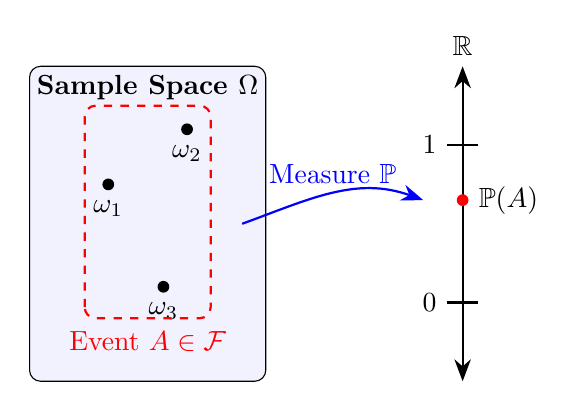
\begin{tikzpicture}[
    > = {Stealth[scale=1.2]},
    box/.style = {draw, rounded corners, minimum width=3cm, minimum height=4cm, align=center},
    ]

    % Sample Space Omega
    \node[box, fill=blue!5] (omega) at (0,0) {};
    \node[anchor=north] at (omega.north) {\textbf{Sample Space $\Omega$}};
    \node[circle, fill=black, inner sep=1.5pt, label=below:$\omega_1$] (w1) at (-0.5, 0.5) {};
    \node[circle, fill=black, inner sep=1.5pt, label=below:$\omega_2$] (w2) at (0.5, 1.2) {};
    \node[circle, fill=black, inner sep=1.5pt, label=below:$\omega_3$] (w3) at (0.2, -0.8) {};
    
    % Event A subset
    \draw[thick, red, dashed, rounded corners] (-0.8, -1.2) rectangle (0.8, 1.5);
    \node[red] at (0, -1.5) {Event $A \in \mathcal{F}$};

    % Real Number Line
    \draw[<->, thick] (4, -2) -- (4, 2) node[above] {$\mathbb{R}$};
    \draw[thick] (3.8, -1) node[left] {$0$} -- (4.2, -1);
    \draw[thick] (3.8, 1) node[left] {$1$} -- (4.2, 1);
    \node[circle, fill=red, inner sep=1.5pt, label=right:$\mathbb{P}(A)$] (pA) at (4, 0.3) {};

    % Mapping Arrow
    \draw[->, thick, blue] (1.2, 0) to[out=20, in=160] node[above] {Measure $\mathbb{P}$} (3.5, 0.3);

\end{tikzpicture}
\end{center}

\subsection{Heuristics and Pitfalls}
\begin{itemize}
    \item \textbf{Pitfall: Confusing "Mutually Exclusive" with "Independent".} Mutually exclusive events ($A \cap B = \emptyset$) can NEVER be independent unless one has a probability of zero. If $A$ happens, $B$ is guaranteed not to happen, meaning they are heavily dependent.
    \item \textbf{Heuristic: "At least one..."} The moment you see "at least one", immediately construct your equation around $1 - \Prob(\text{None})$.
    \item \textbf{Pitfall: The Bose-Einstein Fallacy (Indistinguishable vs Distinguishable).} In probability, identical items (like two dice) must mathematically be treated as \textit{distinguishable} to maintain a uniform probability measure over the sample space. Failing to do so causes one to erroneously assume the sum of 2 is just as likely as the sum of 7.
\end{itemize}

\newpage
% =====================================================================
% PART 5: Conceptual Synthesis and The "Big Picture"
% =====================================================================
\section{Part 5: Conceptual Synthesis and The "Big Picture"}

\subsection{A) Thematic Connections}
The core unifying theme of this chapter is the \textbf{translation of qualitative randomness into quantitative set theory}. Before this chapter, "chance" was an ambiguous concept. By introducing $\sigma$-algebras and mapping them via a measure $\Prob$, we unify counting (combinatorics), logic (Boolean set operations), and analysis (functions). Combinatorics is no longer just "counting"; it is formally defining the cardinality of sub- $\sigma$-algebras in a discrete uniform probability space.

\subsection{B) Forward and Backward Links}
\begin{itemize}
    \item \textbf{Backward Links:} This chapter serves as the direct application of discrete mathematics and basic set theory. The union and intersection operations are identical to logical disjunction (OR) and conjunction (AND) studied in introductory logic.
    \item \textbf{Forward Links:} This specific discrete framing is the foundational bedrock for \textbf{Measure Theory}. In advanced courses, the finite sample space $\Omega$ transitions to $\R$. Because counting permutations becomes impossible with infinities, the discrete sums $\sum \Prob(x)$ are rigorously replaced by the Lebesgue integral $\int_\Omega X \, d\Prob$. Furthermore, understanding sequences of independent events here prepares you for filtrations (accumulating knowledge over time) in Stochastic Calculus.
\end{itemize}

% =====================================================================
% PART 6: Abstract Real-World Modeling (AI, ML, & Quant Finance)
% =====================================================================
\section{Part 6: Abstract Real-World Modeling}

\subsection{Concrete Scenarios}
\begin{enumerate}
    \item \textbf{Quantitative Finance (Derivative Pricing):} The combinatorics of coin-flipping directly maps to the Cox-Ross-Rubinstein (CRR) Binomial Options Pricing Model. The number of paths a stock can take to reach a specific node at expiration is fundamentally $\binom{N}{k}$, representing $k$ "up" movements in $N$ time steps.
    \item \textbf{Machine Learning (Bayesian Networks):} Compound events and partitioning define the structure of Directed Acyclic Graphs (DAGs) in AI. Factorizing a joint probability space using the fundamental rules of sets is what allows algorithms to run efficiently over thousands of variables.
\end{enumerate}

\subsection{Model Problem Setup: The Binomial Lattice in Finance}
Let us formalize a discrete-time stochastic model for pricing a European Call Option using the combinatorial framework established in this homework.

\textbf{State Space and Filtrations:}
Let time be discrete, $t \in \{0, 1, 2, \dots, N\}$. The fundamental sample space of market movements is $\Omega = \{U, D\}^N$, where $U$ signifies the stock moving Up and $D$ signifies Down.
A single sample point is a path $\omega = (X_1, X_2, \dots, X_N) \in \Omega$. 
The stock price at time $N$ is a random variable $S_N : \Omega \to \R^+$ given by:
\[ S_N(\omega) = S_0 \cdot u^{k(\omega)} \cdot d^{N - k(\omega)} \]
where $k(\omega)$ counts the number of times $U$ appears in the path $\omega$, and $u, d$ are the magnitude of up/down market ticks.

\textbf{Measure Transformation:}
Instead of physical probability, Quantitative Finance requires pricing under a \textit{Risk-Neutral Measure} $\mathbb{Q}$. Let $q = \frac{1+r-d}{u-d}$ (where $r$ is the risk-free interest rate). 
The measure $\mathbb{Q}$ assigns the following probability to any path $\omega$ containing exactly $k$ up-moves:
\[ \mathbb{Q}(\omega) = q^k (1-q)^{N-k} \]

\textbf{Combinatorial Optimization:}
The value of a European Call option with strike $K$ is the expected discounted payoff. We group the paths using combinations, just as in the homework! The number of paths resulting in exactly $k$ up moves is $\binom{N}{k}$. Thus, the summation bypasses evaluating all $2^N$ paths and instead evaluates $N+1$ partitions:
\[ C_0 = \frac{1}{(1+r)^N} \sum_{k=0}^{N} \binom{N}{k} q^k (1-q)^{N-k} \max(S_0 u^k d^{N-k} - K, 0) \]
This shows how basic permutations and combinations directly support billion-dollar algorithmic pricing architectures.

\newpage
% =====================================================================
% PART 7: Common Variations and Untested Concepts
% =====================================================================
\section{Part 7: Common Variations and Untested Concepts}

The homework introduces combinations but misses a classical, fundamental technique for combinatorial arrangements regarding \textit{indistinguishable objects in distinct bins}, which is critical in physics (Bose-Einstein statistics).

\subsection{Stars and Bars (Balls and Urns) Theorem}
\textbf{Concept:} How do you find the number of ways to distribute $n$ identical items into $k$ distinct groups (or jobs/bins)? 
Unlike the multinomial partition (which uses distinguishable items), this requires a different logical mapping.

\begin{theorem}
    The number of non-negative integer solutions to $x_1 + x_2 + \dots + x_k = n$ is given by:
    \[ \binom{n + k - 1}{k - 1} \]
\end{theorem}
\begin{proof}[Proof Sketch (Combinatorial)]
    Represent the $n$ items as indistinguishable stars ($\star$). To partition them into $k$ groups, we need to insert $k-1$ vertical bars ($|$) between the stars. 
    The sequence is mapped to a total of $n + (k - 1)$ positions. We simply choose which $k-1$ of these positions will hold the bars. Order does not matter, leading directly to the combination $\binom{n + k - 1}{k - 1}$.
\end{proof}

\begin{example}[Advanced Application]
    You have 10 identical one-dollar bills to give to 4 children. How many ways can this be done if it is possible for a child to receive nothing?
\end{example}
\begin{proof}[Solution]
    Here, $n=10$ (items) and $k=4$ (distinct children).
    \[ \text{Ways} = \binom{10 + 4 - 1}{4 - 1} = \binom{13}{3} = \frac{13 \times 12 \times 11}{3 \times 2 \times 1} = 286 \]
\end{proof}

% =====================================================================
% PART 8: Advanced Diagnostic Testing: "Find the Flaw"
% =====================================================================
\section{Part 8: Advanced Diagnostic Testing: "Find the Flaw"}

Below are 5 seemingly rigorous proofs/solutions containing a subtle, critical logical flaw. Your task as the grader is to identify the error and correct it.

\begin{flaw}[The Additivity Trap]
    \textbf{Problem:} A die is rolled. Let $A = \{2, 4, 6\}$ and $B = \{1, 2, 3\}$. Find $\Prob(A \cup B)$. \\
    \textbf{Flawed Solution:} By Kolmogorov's Axioms, $\Prob(A \cup B) = \Prob(A) + \Prob(B)$. 
    $\Prob(A) = 3/6 = 1/2$. $\Prob(B) = 3/6 = 1/2$. Therefore, $\Prob(A \cup B) = 1/2 + 1/2 = 1$.
\end{flaw}

\begin{flaw}[The Macroscopic Uniformity Assumption]
    \textbf{Problem:} Two fair six-sided dice are rolled. What is the probability that their sum is 7? \\
    \textbf{Flawed Solution:} The possible sums range from 2 to 12. There are 11 possible sums. The sample space is $\Omega = \{2, 3, 4, \dots, 12\}$. Since there are 11 outcomes, the probability of rolling a 7 is exactly $\Prob(7) = 1/11$.
\end{flaw}

\begin{flaw}[Permutation Overcount]
    \textbf{Problem:} A committee of 3 is formed from 10 people. What is the probability that Bob, Alice, and Charlie are chosen? \\
    \textbf{Flawed Solution:} The number of ways to pick 3 people from 10 is $P(10, 3) = 10 \times 9 \times 8 = 720$. The specific event of Bob, Alice, and Charlie is 1 outcome. So the probability is $1/720$.
\end{flaw}

\begin{flaw}[The Subset-Space Paradox]
    \textbf{Problem:} Three fair coins are tossed. We observe that at least one coin landed Heads. What is the probability that all three landed Heads? \\
    \textbf{Flawed Solution:} The sample space for three coins is size 8. The event of 3 Heads ($HHH$) has size 1. Since we know one coin is Heads, the remaining two coins just act independently. $1/2 \times 1/2 = 1/4$.
\end{flaw}

\begin{flaw}[Mutual Exclusivity Implies Independence]
    \textbf{Problem:} In a deck of cards, let $A$ be drawing a Heart, and $B$ be drawing a Spade. Are $A$ and $B$ independent? \\
    \textbf{Flawed Solution:} $A \cap B = \emptyset$ because a card cannot be both a Heart and a Spade simultaneously. Because their intersection is empty, the events have no overlap, meaning they do not interact. Therefore, they are perfectly independent.
\end{flaw}

\vspace{1cm}
\subsection*{Solution Key to "Find the Flaw"}
\begin{enumerate}
    \item \textbf{Flaw:} Axiom 3 only applies to \textit{mutually exclusive} disjoint events. $A$ and $B$ share $\{2\}$, so they are not disjoint. \\ \textbf{Correction:} Use the Inclusion-Exclusion Principle: $\Prob(A \cup B) = \Prob(A) + \Prob(B) - \Prob(A \cap B) = 3/6 + 3/6 - 1/6 = 5/6$.
    \item \textbf{Flaw:} The mapping to the macroscopic sums $\{2 \dots 12\}$ is NOT a uniform measure. The underlying uniform space is $\Omega = \{(1,1), \dots, (6,6)\}$ of size 36. \\ \textbf{Correction:} The event "sum is 7" contains 6 microstates $\{(1,6), (2,5), (3,4), (4,3), (5,2), (6,1)\}$. Prob $= 6/36 = 1/6$.
    \item \textbf{Flaw:} A committee implies order does not matter, but the denominator was calculated using permutations (order matters). This scales the sample space artificially. \\ \textbf{Correction:} Use combinations. $\binom{10}{3} = 120$. Probability is $1/120$. 
    \item \textbf{Flaw:} This is a conditional probability trap that misidentifies the reduced sample space. \\ \textbf{Correction:} The given information "at least one Head" reduces $\Omega$ from 8 down to 7 (eliminating only $TTT$). The event $HHH$ is exactly 1 outcome in this new restricted space. Prob $= 1/7$.
    \item \textbf{Flaw:} Conflating set-theoretic disjointness with statistical independence. \\ \textbf{Correction:} Since they are mutually exclusive, if $A$ occurs, $B$ has a 0\% chance of occurring. $\Prob(B|A) = 0 \neq \Prob(B)$. Therefore, they are highly \textit{dependent}.
\end{enumerate}

\end{document}